\documentclass[tikz,border=4pt]{standalone}
% Estilo común de los diagramas de bloques (se usa con \input en cada standalone)
\usepackage[defaultsans,scale=0.92]{lato}
\usepackage{libertinust1math}
\usepackage{xcolor,amsmath}
\usepackage{tikz}
\usetikzlibrary{positioning,arrows.meta,calc,shapes.geometric}
\usepackage{../../notacion}
\definecolor{ctrlazul}{HTML}{1E5AA8}\definecolor{ctrlnoche}{HTML}{14213D}
\definecolor{ctrlcoral}{HTML}{D1495B}\definecolor{ctrlverde}{HTML}{2A9D8F}
\definecolor{ctrlambar}{HTML}{E09F3E}\definecolor{ctrlgris}{HTML}{5C677D}
\definecolor{ctrlvioleta}{HTML}{6C4AB6}\definecolor{ctrlteal}{HTML}{0F7173}
\tikzset{
  >={Stealth[length=2.4mm]}, every node/.style={font=\small},
  bloque/.style={draw=ctrlnoche,fill=ctrlazul!7,thick,rounded corners=1.5pt,minimum height=9mm,minimum width=13mm,inner sep=4pt},
  suma/.style={draw=ctrlnoche,thick,circle,inner sep=0pt,minimum size=6mm},
  senal/.style={->,thick,draw=ctrlnoche},
  rot/.style={font=\footnotesize,text=ctrlgris},
}

\begin{document}
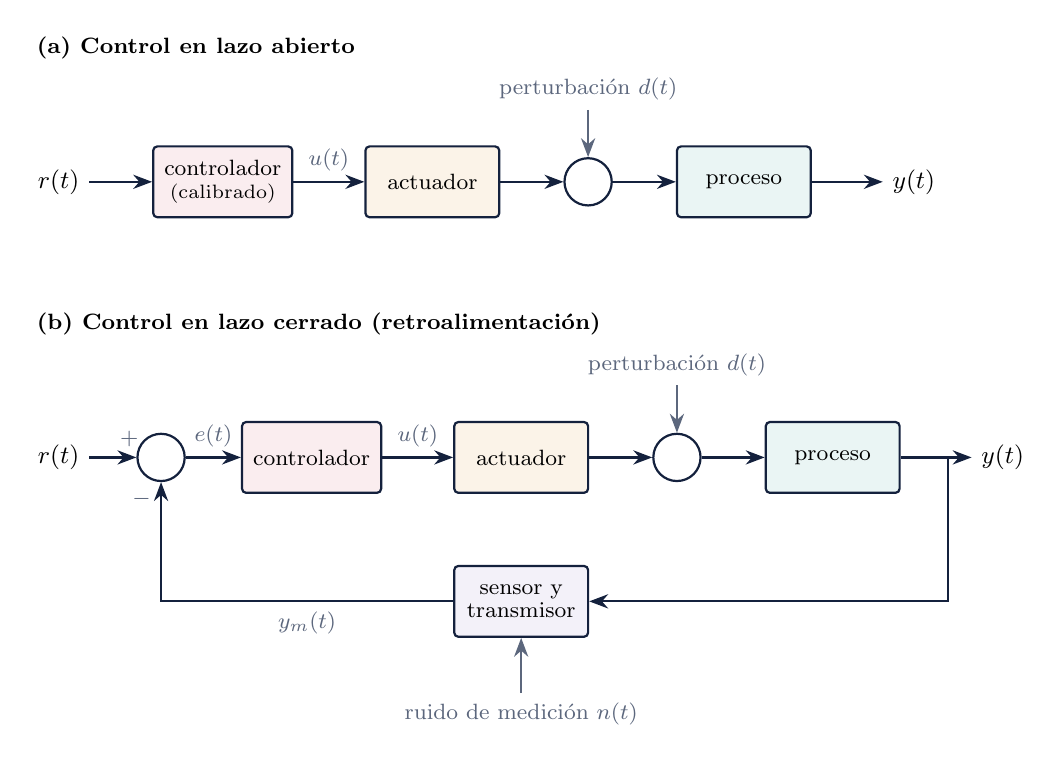
\begin{tikzpicture}[node distance=9mm, b/.style={bloque,minimum width=17mm,font=\footnotesize,align=center}]
  % ---------------- (a) lazo abierto
  \node[font=\footnotesize\bfseries,anchor=west] at (-0.4,1.7) {(a) Control en lazo abierto};
  \node (r0) at (0,0) {$r(t)$};
  \node[b,right=8mm of r0,fill=ctrlcoral!10] (c0) {controlador\\[-1pt]{\scriptsize (calibrado)}};
  \node[b,right=of c0,fill=ctrlambar!12] (a0) {actuador};
  \node[suma,right=8mm of a0] (s0) {};
  \node[b,right=8mm of s0,fill=ctrlverde!10] (p0) {proceso};
  \node[right=9mm of p0] (y0) {$y(t)$};
  \node[above=6mm of s0,rot] (d0) {perturbación $d(t)$};
  \draw[senal] (r0)--(c0); \draw[senal] (c0)--node[above,rot]{$u(t)$}(a0);
  \draw[senal] (a0)--(s0); \draw[senal] (s0)--(p0); \draw[senal] (p0)--(y0);
  \draw[senal,draw=ctrlgris] (d0)--(s0);
  % ---------------- (b) lazo cerrado
  \begin{scope}[yshift=-3.5cm]
  \node[font=\footnotesize\bfseries,anchor=west] at (-0.4,1.7) {(b) Control en lazo cerrado (retroalimentación)};
  \node (r) at (0,0) {$r(t)$};
  \node[suma,right=6mm of r] (S) {};
  \node[b,right=7mm of S,fill=ctrlcoral!10] (c) {controlador};
  \node[b,right=of c,fill=ctrlambar!12] (a) {actuador};
  \node[suma,right=8mm of a] (s1) {};
  \node[b,right=8mm of s1,fill=ctrlverde!10] (p) {proceso};
  \coordinate[right=6mm of p] (o); \node[right=3mm of o] (y) {$y(t)$};
  \node[above=6mm of s1,rot] (d) {perturbación $d(t)$};
  \node[b,below=9mm of a,fill=ctrlvioleta!8] (se) {sensor y\\[-1pt]transmisor};
  \node[below=7mm of se,rot] (n) {ruido de medición $n(t)$};
  \draw[senal] (r)--node[pos=0.85,above,rot]{$+$}(S);
  \draw[senal] (S)--node[above,rot]{$e(t)$}(c);
  \draw[senal] (c)--node[above,rot]{$u(t)$}(a);
  \draw[senal] (a)--(s1); \draw[senal] (s1)--(p);
  \draw[thick,draw=ctrlnoche] (p)--(o); \draw[senal] (o)--(y);
  \draw[senal,draw=ctrlgris] (d)--(s1);
  \draw[senal] (o)|-(se);
  \draw[senal,draw=ctrlgris] (n)--(se);
  \draw[senal] (se)-|node[pos=0.25,below,rot]{$y_m(t)$}node[pos=0.93,left,rot]{$-$}(S);
  \end{scope}
\end{tikzpicture}
\end{document}
